\documentclass[student, noshadow, lsr, english, aspectratio=169, t]{ITR_LSR_slides}

\setbeamertemplate{frametitle}{%
  \vspace{0.3cm}% Space between top edge and title
  \if@center
    \begin{centering}
      \textbf{\vphantom{Sp}\insertframetitle\vphantom{Sp}}
      \par
    \end{centering}
  \else
    \textbf{\vphantom{Sp}\insertframetitle\vphantom{Sp}}
    \par
  \fi
  \vspace{0.3cm}% Space between title and content
}

% Add top margin to frames without titles
\addtobeamertemplate{frame begin}{%
  \ifx\insertframetitle\@empty
    \vspace{0.8cm}% Space at top of frames without titles
  \fi
}{}

\addbibresource{ref.bib}
\graphicspath{{pics/}{logos/}}

\title{Analysis and Control of Time-Varying and Perturbed Systems}
\presenter{Keno Bürger}
\typeofpres{Advanced Nonlinear Control}

\usepackage{multirow}
\usepackage{graphicx}
\usepackage[T1]{fontenc}
\usepackage{lmodern}
\usepackage{tabularx}
\usepackage{enumitem}
\usepackage{adjustbox}
\usepackage{array}
\usepackage{booktabs}
\usepackage{makecell}
\usepackage{hyperref}

% Load hyperref as the last package before document begins
\hypersetup{
	pdftitle={Advanced Nonlinear Control: Lyapunov Stability and Perturbations},
	pdfauthor={Keno Bürger},
	pdfsubject={Nonlinear Control Theory},
	pdfkeywords={Lyapunov stability, exponential stability, boundedness, ultimate boundedness, perturbations, nonlinear control},
	pdfcreator={LaTeX with Beamer},
	pdfproducer={pdfTeX},
}

% Fix for potential BOM or invisible characters
\begin{document}

\begin{frame}
    \titlepage
\end{frame}


%%%%%%%%%%%%%%%%%%%%%%%%%%%%%%%%%%%%%%%%%%%%%%%%%%%%%%
\section{Introduction}

\begin{frame}
    \frametitle{Main Objective}

    \textbf{Based on:}
    \begin{itemize}
        \item \textit{Nonlinear Control} (Ch. 4): Time-varying and perturbed systems
        \item \textit{Nonlinear Systems} (Ch. 9, 11.5): Stability under perturbations
    \end{itemize}
	\vspace{0.5cm}
    \textbf{Objective:}
    \begin{itemize}
		\item Formulate practical and broadly applicable stability conditions
        \item Analyze stability under \textbf{vanishing perturbations} using comparison functions
        \item Study ultimate boundedness for systems with \textbf{non-vanishing perturbations}
        % \item Apply Lyapunov-based methods for robust analysis of nonlinear, time-varying systems
    \end{itemize}
\end{frame}

\begin{frame}
	\frametitle{Lyapunov Theory for Time-Varying Systems}
	% \begin{itemize}
	% 	\item Definition of Uniform, Asymptotic and exponential stability \cite{muennighoff_s1_2025}
	% 	\item Application of Lyapunov Stability Theorems
	% \end{itemize}
	\textbf{Assumptions:}
	\begin{itemize}
		\item Origin $\underline{x}=0$ is an equilibrium point
		\item Lyapunov function $V(t,\underline{x})$ is continuously differentialbe, positive definite and radially unbounded
		\item Derivative of Lyapunov function is negative definite
	\end{itemize}
	\vspace{0.5cm}
	\textbf{Globally uniformly exponentially stable:}
	\begin{align*}
		\exists\, c_i, \alpha > 0: & \; c_1\left\|\underline{x}\right\|^\alpha \leq V(t,\underline{x}) \leq c_2\left\|\underline{x}\right\|^\alpha  \\
		& \dot{V}(t,\underline{x}) \leq -c_3\|\underline{x}\|^\alpha
	\end{align*}
\end{frame}

\begin{frame}
	\frametitle{Boundedness and Ultimate Boundedness}
	% \begin{itemize}
	% 	\item Differences
	% 	\item Build bridge to non vanishing and vanishing perturbations
	% \end{itemize}
	\begin{figure}
		\centering
		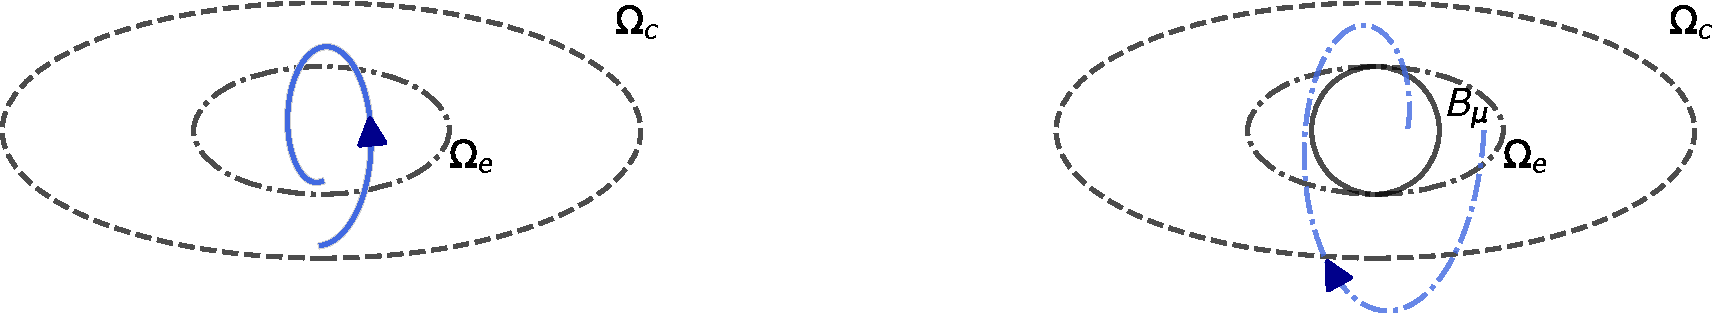
\includegraphics[width=\textwidth]{ultimate_boundedness_rotated.pdf}
		\caption{}
		\label{fig:boundedness_vs_ultimate_boundedness}
	\end{figure}
	\vspace{-1cm}
	\begin{columns}[t,totalwidth=\textwidth]
        \column{0.47\textwidth}
		\textbf{Boundedness:}
		\begin{align*}
			\|\underline{x}(t_0)\| \leq \alpha \Rightarrow \|\underline{x}(t)\| \leq \beta,
			\\ c>0, \alpha\in(0,c),\, \beta>0,\,\forall\, t \geq t_0
		\end{align*}

        \column{0.47\textwidth}
		\textbf{Ultimate Boundedness:}
		\begin{align*}
			\|\underline{x}(t)\| \leq b 
			\\ \forall\, t \geq t_0+T
		\end{align*}
    \end{columns}
\end{frame}

% \begin{frame}
% 	\frametitle{Perturbation Models: Vanishing vs. Non-Vanishing}
% 	\textbf{Motivation:} Real-world systems are subject to time dependence, modelling errors and external disturbances

% 	\vspace{0.5em}
% 	\textbf{System:} $\dot{\underline{x}} = f(\underline{x}) + g(\underline{x}, t)$
% 	\begin{itemize}
% 		\item $f$ locally Lipschitz
% 		\item $g$ piecewise continuous in $t$, locally Lipschitz in $\underline{x}$
% 		\item $g$ generally unknown, but bounded
% 	\end{itemize}

% 	\vspace{0.5em}
% 	\textbf{Vanishing Perturbation:} $g(\underline{x}, t) \to 0$ as $\underline{x} \to 0$ \\
% 	$\Rightarrow$ Exponential stability of the origin is preserved (robustness)

% 	\vspace{0.3em}
% 	\textbf{Non-Vanishing Perturbation:} $g(\underline{x}, t) \not\to 0$ as $\underline{x} \to 0$ \\
% 	$\Rightarrow$ Solutions remain bounded (ultimate boundedness)
% \end{frame}


\begin{frame}
	\frametitle{Understanding Perturbation Types}

	\textbf{Motivation:} Real-world systems are subject to time dependence, modelling errors and external disturbances
	
	\vspace{0.5cm}
	\textbf{General System Form:} 
	\[\dot{\underline{x}} = f(\underline{x}) + g(\underline{x}, t)\]
	
	\vspace{0.5cm}
	\begin{columns}[t,totalwidth=\textwidth]
        \column{0.48\textwidth}
		\textbf{Vanishing Perturbation:}
		\begin{itemize}
			\item $g(\underline{x}, t) \to 0$ as $\underline{x} \to 0$
			\item Preserves exponential stability
			\item Examples: modeling errors
		\end{itemize}

        \column{0.48\textwidth}
		\textbf{Non-Vanishing Perturbation:}
		\begin{itemize}
			\item $g(\underline{x}, t) \not\to 0$ as $\underline{x} \to 0$
			\item Leads to ultimate boundedness
			\item Examples: constant disturbances
		\end{itemize}
    \end{columns}
\end{frame}


%%%%%%%%%%%%%%%%%%%%%%%%%%%%%%%%%%%%%%%%%%%%%%%%%%%%%
\section{Vanishing Perturbations}

\begin{frame}
	\frametitle{Lyapunov Stability Theorems}
	% \begin{itemize}
	% 	\item Exponential Stability
	% 	\item Highlight challenges with this approach
	% \end{itemize}
	\textbf{Assumptions:}
	\begin{itemize}
		\item Origin $\underline{x}=0$ is an exponentially stable equilibrium point
		\item Perturbation vanishes
		\item Lyapunov function $V(t,\underline{x})$ is continuously differentialbe, positive definite and radially unbounded
	\end{itemize}
	\vspace{0.5cm}
	\textbf{Globally Uniformly Exponentially Stable Equilibrium:}
	\begin{align*}
		\frac{\partial V}{\partial t}+\frac{\partial V}{\partial \underline{x}}f(\underline{x}) \leq c_3\|\underline{x}\|^2 \text{ and }\|\frac{\partial V}{\partial \underline{x}}\| \leq c_4\|\underline{x}\|
	\end{align*}
	\begin{align*}
		\|g(\underline{x},t)\| \leq \gamma\|\underline{x}\| \text{ with }0\leq\gamma(t)<\frac{c_3}{c_4}
	\end{align*}

\end{frame}

\begin{frame}
	\frametitle{Comparison Lemma – Example}

	\textbf{System:}
	\begin{align*}
		\dot{\underline{x}} = -a\,\underline{x}(t) + g(t, \underline{x}), \quad \underline{x}(0) = 0, \quad a > 0
	\end{align*}

	\textbf{Assumptions:}
	\begin{itemize}
		\item $\underline{x}(t) \geq 0 \quad \forall\, t \geq 0$
		\vspace{0.3em}
		\item $g(t, \underline{x}) \leq b\,\underline{x}(t) \quad \forall\, x \geq \underline{x} \geq 0$
	\end{itemize}

	\textbf{Integral Condition:}
	\begin{align*}
		\underline{x}(t) \leq \underline{x}_0 + \int_{t_0}^{t} \gamma(\tau)\, d\tau 
		= \underline{x}_0 + \int_{t_0}^{t} [-a\,\underline{x}(\tau) + b\,\underline{x}(\tau)]\, d\tau
	\end{align*}

	\textbf{Bound for Derivative:}
	\begin{align*}
		\dot{\underline{x}}(t) \leq -a\,\underline{x}(t) + b\,\underline{x}(t) = -(a - b)\,\underline{x}(t)
	\end{align*}
\end{frame}

\begin{frame}
	\frametitle{Comparison Lemma – Example}

	\begin{align*}
		\underline{x}(t) \leq \underline{x}_0 + \int_{t_0}^{t} \dot{\underline{x}}(\tau)\, d\tau 
		\leq \underline{x}_0 - (a - b) \int_{t_0}^{t} \underline{x}(\tau)\, d\tau
	\end{align*}

	If $(a - b)\,\underline{x}$ is continuous, positive definite, and non-decreasing, then:
	\begin{align*}
		\lim_{t \to \infty} \underline{x}(t) = 0
	\end{align*}

	which ensures that the system loses more than it gains.

	\vspace{0.5em}
	Furthermore, exponential decay is guaranteed:
	\begin{align*}
		\underline{x}(t) \leq \underline{x}_0\, e^{-(a - b)t}
	\end{align*}
	% from differntial equations
\end{frame}


% \begin{frame}
% 	\frametitle{Comparison Functions}
% 	% \begin{itemize}
% 	% 	\item Differences and Benefits of this approach
% 	% 	\item Corollary 1
% 	% \end{itemize}
% 	\textbf{Assumptions:}
% 	\begin{itemize}
% 		\item Origin $\underline{x}=0$ is an exponentially stable equilibrium point
% 		\item Perturbation vanishes
% 	\end{itemize}
% 	\vspace{0.5cm}
% 	\textbf{Exponential Stability:}
% 	\begin{align*}
% 		\|g(\underline{x},t)\| \leq \gamma(t)\|\underline{x}\| \text{ with }\int_{t_0}^{t}\gamma(\tau)\,d\tau<\epsilon(t-t_o)+\eta
% 	\end{align*}
% 	\begin{align*}
% 		\text{with } \epsilon < \frac{c_1c_3}{c_2c_4}
% 	\end{align*}
% \end{frame}

% \begin{frame}
% 	\frametitle{Example: Linear Time-Varying System}
% 	% \begin{itemize}
% 	% 	\item $\dot{\underline{x}}=[A(T)+B(t)]\underline{x}$
% 	% 	\item Lyapunov function $V(t,\underline{x})$ is positive definite and derivative negative definite
% 	% 	\item $g(t,\underline{x}) = B(t)\underline{x} \Rightarrow \|g(t,\underline{x})\| \leq \|B(t)\| \cdot \|\underline{x}\| = \gamma(t) \|\underline{x}\|$
% 	% 	\item $\int_{t_0}^{t}\gamma(\tau)\,d\tau<\epsilon(t-t_o)+\eta$
% 	% 	\item[$\Rightarrow$] Exponetial stability of nominal system is preserved under vanishing perturbations
% 	% \end{itemize}
% 	\textbf{Perturbed Linear Time-Varying System:}
% 	\begin{align*}
% 		\dot{\underline{x}}=[A(t)+B(t)]\underline{x}
% 	\end{align*}
% 	\textbf{Assumptions:}
% 	\begin{itemize}
% 		\item $A(t)$ is uniformly bounded
% 		\item Origin of nominal system is uniformly exponentially stable
% 		\item $B(t) \rightarrow 0$ as $t\rightarrow\infty$
% 		\item Lyapunov function $V(t,\underline{x})$ is positive definite and derivative negative definite
% 	\end{itemize}
% 	\begin{align*}
% 		g(t,\underline{x}) = B(t)\underline{x} \Rightarrow \|g(t,\underline{x})\| \leq \|B(t)\| \cdot \|\underline{x}\| = \gamma(t) \|\underline{x}\|
% 	\end{align*}
% 	$\Rightarrow$ Exponential stability of nominal system is preserved under vanishing perturbations
	
% \end{frame}

%%%%%%%%%%%%%%%%%%%%%%%%%%%%%%%%%%%%%%%%%%%%%%%%%%%%%
\section{Non-Vanishing Perturbations}

\begin{frame}
	\frametitle{Lyapunov-Based Conditions for Boundedness}

	\textbf{Assumptions:}
	\begin{itemize}
		\item $\underline{x} = 0$ is exponentially stable for the nominal system
		\item Non-vanishing, bounded perturbation $g(\underline{x}, t)$
		\item Lyapunov function $V(t, \underline{x})$ is positive definite and radially unbounded
		\item Perturbation bound:
		\begin{align*}
			\|g(\underline{x}, t)\| \leq \delta < \frac{c_3}{c_4} \sqrt{\frac{c_1}{c_2}}\, \theta r, \quad \theta \in (0,1),\ r > 0
		\end{align*}
	\end{itemize}
\end{frame}


\begin{frame}
	\frametitle{Lyapunov-Based Conditions for Boundedness}

	\textbf{Exponential Stability:} \\
	For all initial conditions satisfying $\|\underline{x}(t_0)\| \leq \sqrt{c_1/c_2} \, r$:
	\begin{align*}
		\|\underline{x}(t)\| \leq k\, e^{-\gamma (t - t_0)} \|\underline{x}(t_0)\|, \quad t_0 \leq t \leq t_0 + T
	\end{align*}

	\textbf{Ultimate Boundedness:}
	\begin{align*}
		\|\underline{x}(t)\| \leq b \quad \forall\, t \geq t_0 + T
	\end{align*}

	\textbf{Parameters:}
	\begin{align*}
		k = \sqrt{\frac{c_2}{c_1}}, \quad \gamma = \frac{(1 - \theta)c_3}{2c_2}, \quad b = \frac{c_4}{c_3}k \frac{\delta}{\theta}
	\end{align*}
\end{frame}

\begin{frame}
	\frametitle{Example: Bounded Disturbance Response}

	\textbf{System:}
	\begin{align*}
		\dot{x}_1 &= x_2 \\ % postion
		\dot{x}_2 &= -2x_1 - 3x_2 + d, \quad |d| \leq \delta % velocity
	\end{align*}

	\textbf{Interpretation:}
	\begin{itemize}
		\item Mass-spring-damper system with constant external force
		\item Nominal system ($d = 0$): exponentially stable
	\end{itemize}

	\vspace{0.3em}

	\textbf{Lyapunov Candidate:} $V(\underline{x}) = \underline{x}^T P \underline{x}$

	\vspace{0.3em}
	\begin{itemize}
		\item $P > 0$ solves $A^T P + P A = -Q$, with $Q = I$
		\item $A = \begin{bmatrix} 0 & 1 \\ -2 & -3 \end{bmatrix}$
	\end{itemize}

	\vspace{0.3em}
	\textbf{Bounds:} \quad $c_1 \|\underline{x}\|^2 \leq V(\underline{x}) \leq c_2 \|\underline{x}\|^2$
\end{frame}


\begin{frame}
	\frametitle{Example: Bounded Disturbance Response}

	\textbf{Lyapunov Derivative:}
	\[
		\dot{V} \leq -c_3 \|\underline{x}\|^2 + c_4 \delta \|\underline{x}\|
	\]

	\textbf{Compare to:}
	\[
		\dot{V} \leq -c_3 \|\underline{x}\|^2 + c_4 \|g(\underline{x}, t)\| \|\underline{x}\|
	\]

	\textbf{Boundedness Condition:}
	\[
		\|g(\underline{x}, t)\| \leq \delta < \frac{c_3}{c_4} \sqrt{\frac{c_1}{c_2}} \theta r, \quad \theta \in (0,1)
	\]

	\vspace{0.3em}
	\textbf{Then:}
	\begin{itemize}
		\item $\|\underline{x}(t)\| \leq b$ for $t \geq t_0 + T$
		\item $b = \dfrac{c_4}{c_3} k \dfrac{\delta}{\theta}, \quad k = \sqrt{c_2/c_1}, \quad \gamma = \dfrac{(1 - \theta)c_3}{2c_2}$
	\end{itemize}

	\vspace{0.3em}
	\textbf{Conclusion:} State converges to a ball around the origin; size scales with $\delta$
\end{frame}




%%%%%%%%%%%%%%%%%%%%%%%%%%%%%%%%%%%%%%%%%%%%%%%%%%
\section{Summary and Discussion}

% \begin{frame}
% 	\frametitle{Conceptual Links Between Sections}
% 	\begin{itemize}
%         \item \textbf{Lyapunov Functions:} Central in both cases, quantify energy and decay
%         \item \textbf{Main Difference:} Convergence to origin vs. convergence to a bounded set
%         \item \textbf{Comparison Lemma:} Powerful for estimating solution bounds in both cases
%         \item \textbf{Ultimate Boundedness:} Reflects robustness, common in practical control
%         \item \textbf{Design Implication:} Small perturbations can be tolerated if decay is fast; persistent ones require constraint-aware design
%     \end{itemize}

%     \vspace{0.5em}
%     \textbf{Takeaway:} Both frameworks enhance system analysis in the presence of uncertainty. Knowing the type of perturbation guides appropriate control strategies.
% \end{frame}

% \begin{frame}
%     \frametitle{Benefits and Drawbacks of Lyapunov-Based Analysis}

%     \textbf{Benefits}
%     \begin{itemize}
%         \item \text{General applicability:} %Works for nonlinear, time-varying, and perturbed systems
%         \item \text{Rigorous and systematic:}% Provides sufficient conditions for stability and boundedness
%         \item \text{Insightful design tool:} %Helps in controller synthesis and robustness analysis
%         \item \text{Comparison lemma:}% Enables practical bounding of trajectories without solving the system
%         \item \text{Handles uncertainty:}% Applicable to both modeling errors (vanishing) and disturbances (non-vanishing)
%     \end{itemize}

%     \textbf{Drawbacks}
%     \begin{itemize}
%         \item \text{Constructing Lyapunov functions is hard:}% No general method for nonlinear systems
%         \item \text{Results are conservative:}% Conditions are sufficient but not necessary
%         \item \text{Limited to local regions:}% Stability often guaranteed only locally unless global bounds are proven
%         \item \text{Quantitative bounds may be loose:}% Worst-case growth rate assumptions can overestimate the effect of perturbations
%     \end{itemize}
% \end{frame}

% \begin{frame}
%     \frametitle{Summary: Insights and Tradeoffs}
%     \begin{columns}[t]
%         \column{0.48\textwidth}
%         \textbf{Conceptual Insights}
%         \begin{itemize}
%             \item Lyapunov methods unify time-varying and perturbed stability analysis
%             \item Key difference: convergence to origin vs. convergence to a bound
%             \item Ultimate boundedness reflects robustness in practical systems
%         \end{itemize}

%         \column{0.48\textwidth}
%         \textbf{Benefits \& Limitations}
%         \begin{itemize}
%             \item Systematic and broadly applicable
%             \item But: Lyapunov construction is hard
%             \item Often conservative; usually local
%         \end{itemize}
%     \end{columns}
%     \vspace{1em}
%     \textbf{Takeaway:} \\
% 	Exponential stability of a nominal system can ensure robust behaviour in the presence of perturbations, but only if the perturbation is appropriately characterised.

% \end{frame}

\begin{frame}
    \frametitle{Key Insights and Practical Implications}
    
    \textbf{Theoretical Insights:}
    \begin{itemize}
        \setlength{\itemsep}{8pt}
        \item Lyapunov methods unify analysis of time-varying and perturbed systems
        \item Perturbation type determines achievable stability properties
        \item Ultimate boundedness reflects real-world system robustness
    \end{itemize}
    
    \vspace{0.8cm}
    \textbf{Design Implications:}
    \begin{itemize}
        \setlength{\itemsep}{8pt}
        \item Small, vanishing perturbations: maintain exponential convergence
        \item Persistent disturbances: design for bounded operation
        \item Robustness requires appropriate perturbation characterization
    \end{itemize}
\end{frame}




%%%%%%%%%%%%%%%%%%%%%%%%%%%%%%%%%%%%%%%%%%%%%%%%%%%%%
\appendix

\begin{frame}[allowframebreaks]
    \frametitle{References}
    \nocite{*} 
    \printbibliography[heading=none]
\end{frame}

\end{document}
